%%%%%%%%%%%%%%%%%%%%%%%%%%%%%%%%%%%%%%%%%%%%%%
\section{Fossil dating}
%%%%%%%%%%%%%%%%%%%%%%%%%%%%%%%%%%%%%%%%%%%%%%

\begin{frame}{And what about this guy?}
\includegraphics[width=0.5\textwidth]{Homo_naledi.jpg}
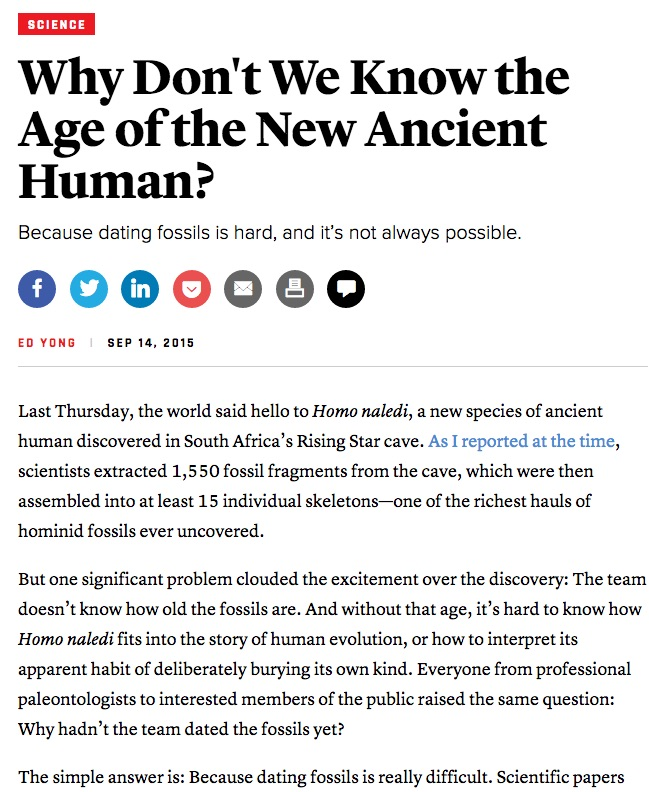
\includegraphics[width=0.5\textwidth]{Atlantic_Homo_naledi.jpg}

\bigskip{}



\end{frame}

\begin{frame}{Can we date fossils using Bayesian phylogenetics? }

Given:
\begin{itemize}
\item A reference set of fossils of known age, and
\item A morphological characterization for reference fossils, and
\item The fossilized birth-death model of sampled ancestor trees
\item A ``clock-like'' model of morphological evolution 
\item A morphological characterization of a related focal fossil of unknown age 
\end{itemize}

{\bf Can the age of the focal fossil be estimated using Bayesian phylogenetic inference?}

\medskip{}

We tested this hypothesis by using the penguin data set. For each of the 36 fossils in turn, we discarded the age information of the focal fossil to mimic the scenario where the age was unknown, and sought to estimate its age using the reference 35 fossils as the reference set. 

\end{frame}


\begin{frame}{Estimating the phylogenetic age of a fossil}
\begin{figure}
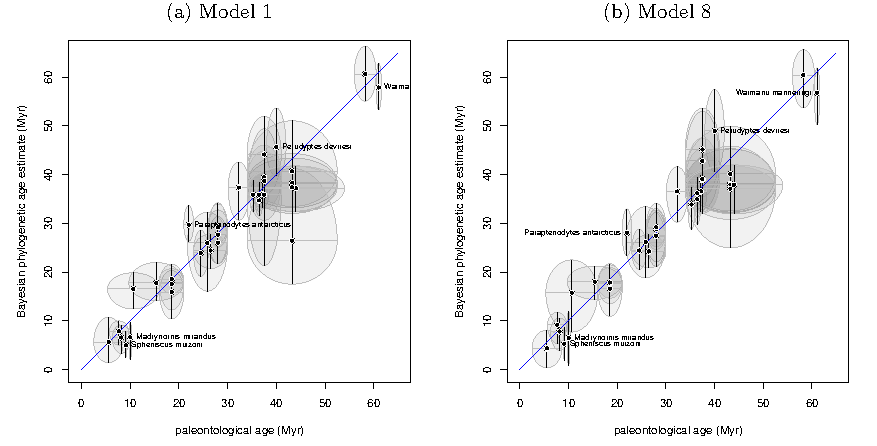
\includegraphics[width=\textwidth]{../Figure1.pdf}
\end{figure}
Bayesian phylogenetic age estimates for each of 36 penguin fossils plotted against their palaeontological age estimates, under two alternative evolutionary models. 
The blue line shows the $x=y$. If the vertical line doesn't cross $x=y$, then the midpoint of the geological range is not in the phylogenetic 95\% HPD. 
\end{frame}

\begin{frame}
\begin{figure}
\includegraphics[width=\textwidth]{../8_penguins_eNprior/8_fossilDatingHist_younger_wide.pdf}
\end{figure}
Marginal posterior density plots for the phylogenetic age estimate of each of the 18 penguin fossils younger than 30 Myr using \Mrelaxed{}. Red boxes are the superimposed age ranges derived from geological data.
\end{frame}

\begin{frame}
\begin{figure}
\includegraphics[width=\textwidth]{../8_penguins_eNprior/8_fossilDatingHist_older_wide.pdf}
\end{figure}
Marginal posterior density plots for the phylogenetic age estimate of each of the 18 penguin fossils older than 30 Myr using \Mrelaxed{}. Red boxes are the superimposed age ranges derived from geological data.
\end{frame}

\begin{frame}
\begin{figure}
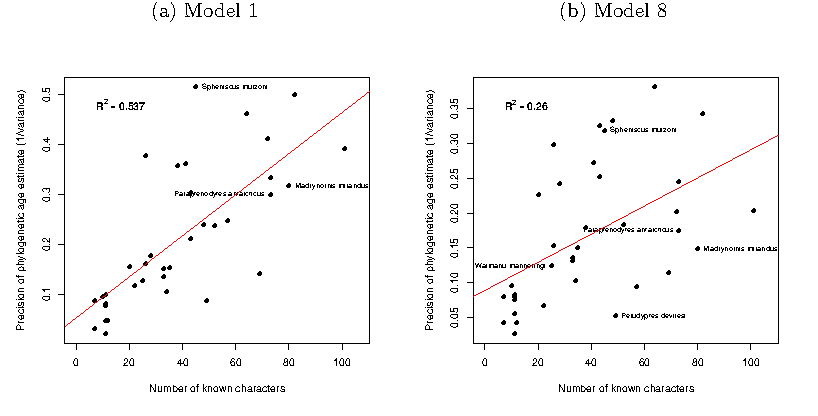
\includegraphics[width=\textwidth]{../Figure2.pdf}
\end{figure}
A plot of the number of non-ambiguous morphological sites for the taxon against the precision of the phylogenetic age for (a) \Mstrict{} and (b) \Mrelaxed{} (i.e. the precision is 1/variance in the marginal posterior distribution of the age).
\end{frame}

\begin{frame}
\frametitle{Comparison of age \& BF estimates between models}
\begin{figure}%
\centering
\subfigure[Estimated phylogenetic age of \Mstrict{} against \Mrelaxed{}.]{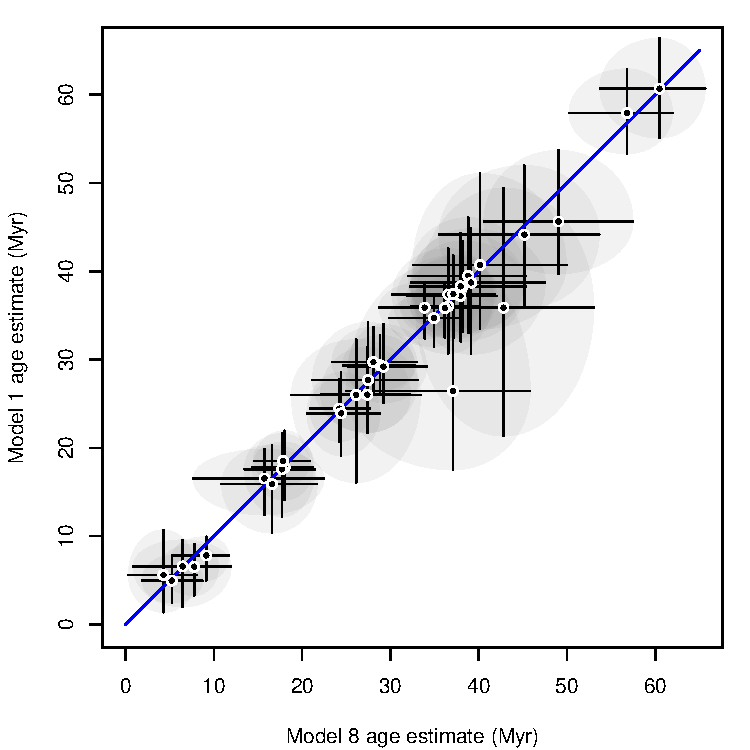
\includegraphics[width=0.45\textwidth]{../compareAgeM1M8.pdf}}\qquad
\subfigure[Regression of Bayes factor (BF) for palaeontological range of \Mstrict{} against \Mrelaxed{}.]{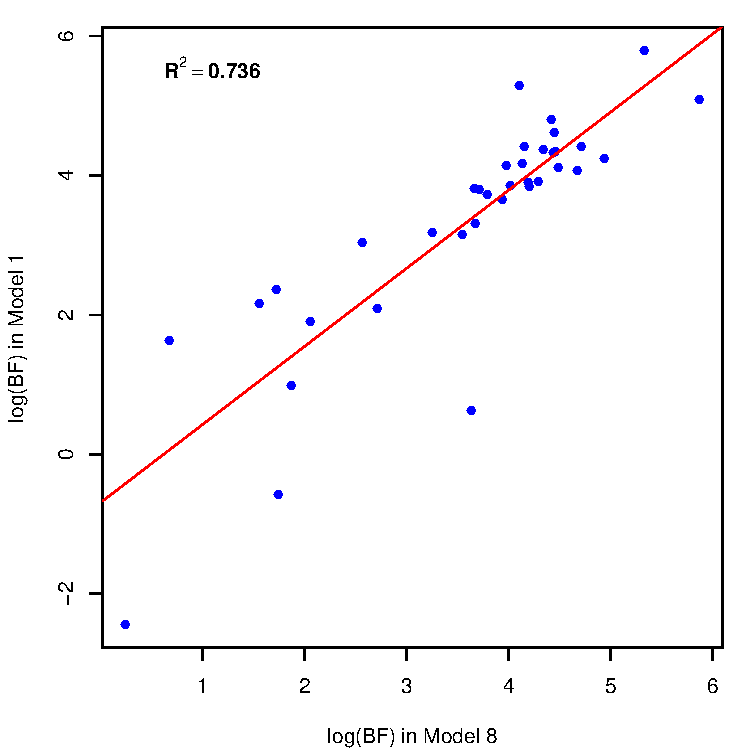
\includegraphics[width=0.45\textwidth]{../compareBFM1M8.pdf}}\\
\label{fig:compareM1M8ab}
\end{figure}
\end{frame}

\begin{frame}
\frametitle{Comparison of probability \& error between models}
\begin{figure}%
\centering
\subfigure[Regression of posterior probability of palaeontological range of \Mstrict{} against \Mrelaxed{}.]{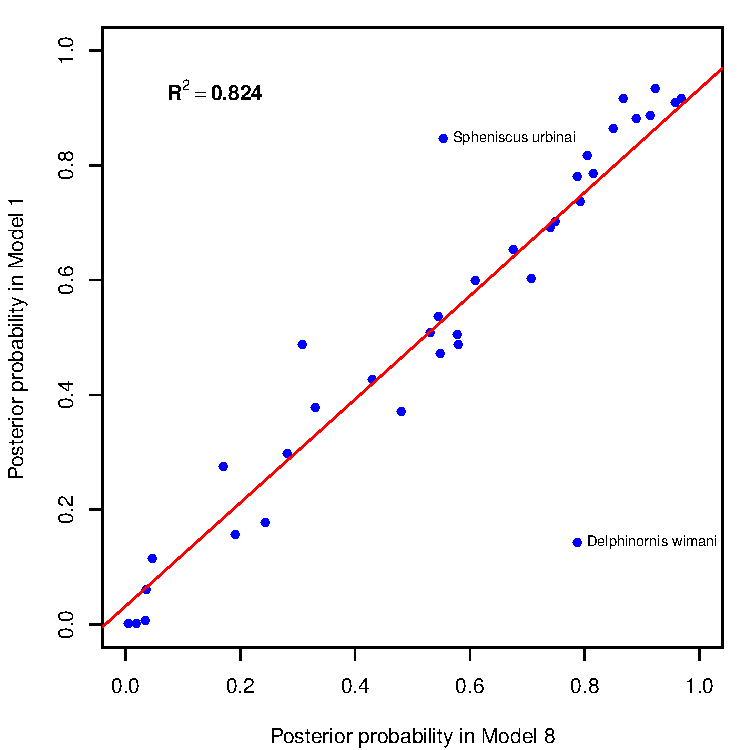
\includegraphics[width=0.45\textwidth]{../comparePostM1M8.pdf}}\qquad
\subfigure[Regression of error in estimated phylogenetic age of \Mstrict{} against \Mrelaxed{}.]{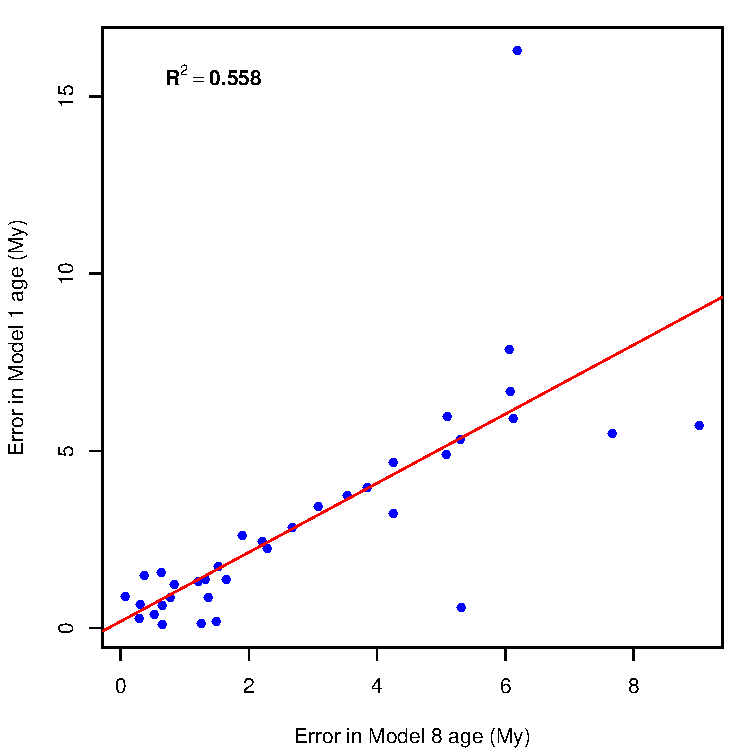
\includegraphics[width=0.45\textwidth]{../compareErrorM1M8.pdf}}\\
\label{fig:compareM1M8cd}
\end{figure}
\end{frame}
